\chapter{API REST}
\label{capapi}

Este capitulo esta destinado a los desarrolladores que deseen interactuar con el Janu Provisioning API, para realizar aprovisionamientos autom'aticos desde cualquier plataforma de desarrollo. Con el API de aprovisionamiento se podr'a crear ambientes y m'aquinas virtuales personalizadas, realizar configuraciones y administrar los recursos f'isicos y virtuales de manera program'atica.

\section{Provisioning API conceptos}
Janu Provisioning esta construido sobre seis conceptos:

\begin{description}
\item[Nodes] Un nodo puede ser cualquier m'aquina f'isica o virtual, los nodos est'an destinados a ser administrados por el software de aprovisionamiento, manteniendo comunicaci'on con el servidor central.
\item[Appliances] Un appliance es una unidad l'ogica de software, puede ser una m'aquina virtual o la instalaci'on de un software dentro de una m'aquina virtual.
\item[Enviroments] Un enviroment representa un ambiente virtual computacional, compuesto de dos o m'as appliances.
\item[LogManager] El logmanager es una unidad l'ogica que comprende el manejo de logs enviados desde los appliances.
\item [Archetypes] Los arquetipos comprenden las caracter'isticas, comportamientos y pol'iticas de los ambientes virtuales y los appliances. 
\item [Users] Los usuarios definen los permisos sobre los nodos, los appliances y el sistema en general.
\end{description}

\section{Provisioning API data model}
Un recurso es un entidad de datos individual con un 'unico identificador. Janu Provisioning API opera con seis tipos de recursos:

\begin{description}
\item [Nodes resource] Representa un nodo; un nodo es un contenedor de appliances.	
\item [LogManage resource] Representa un log. 
\item [Appliances resource] Representa un appliance; un appliance puede ser hijo de un ambiente virtual (enviroment).
\item[Enviroments resource] Representa un ambiente virtual.
\item [Archetypes resource] Representa un arquetipo; un arquetipo define el comportamiento de los ambientes virtuales y los appliances.
\item [Users resource]  Representa un usuario; un usuario es usado para identificar quien tiene autorizaci'on y permiso para acceder a los nodos, sus appliances y el sistema.
\end{description}

%\begin{figure}[hbp]
%  \centering
%  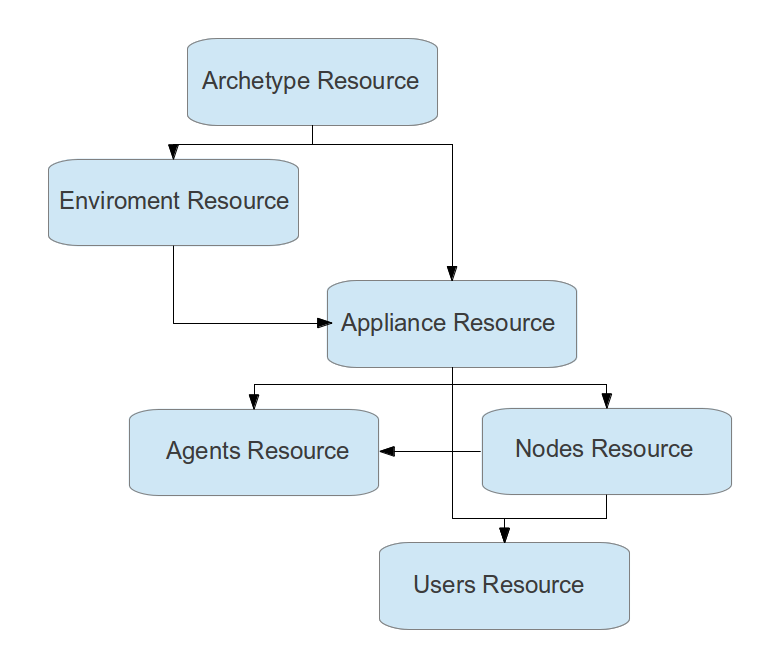
\includegraphics[scale=0.45]{content/fig/RelationshipsBetweenResources}
%  \caption{Visión de las relaciones entre recursos}
%  \label{fig:caption-bottom}
%\end{figure}